\section{Theorie}
\label{sec:Theorie}

Im Rahmen der klassischen Elektrodynamik wird Licht als elektromagnetische Welle beschrieben.
Deshalb kann auch für Licht das wellentypsiche Phänomen der Beugung beobachtet werden,
bei dem sich das Licht in Bereichen ausbreitet, die in der geometrischen Optik nicht zugänglich sind.
Beugung tritt jedoch nur auf, wenn das Objekt, auf das das Licht trifft, Abmessungen in der Größe der Wellenlänge $\lambda$ hat.
Mit Hilfe des Interferenzeffekts und des Huygensschen Prinzips
(Von jedem Punkt einer Wellenfront gehen kreisförmige Elementarwellen aus, die sich überlagern und deren Einhüllende eine neue Wellenfront bildet.)
kann die Beugung erklärt werden.
\begin{figure}
  \centering
  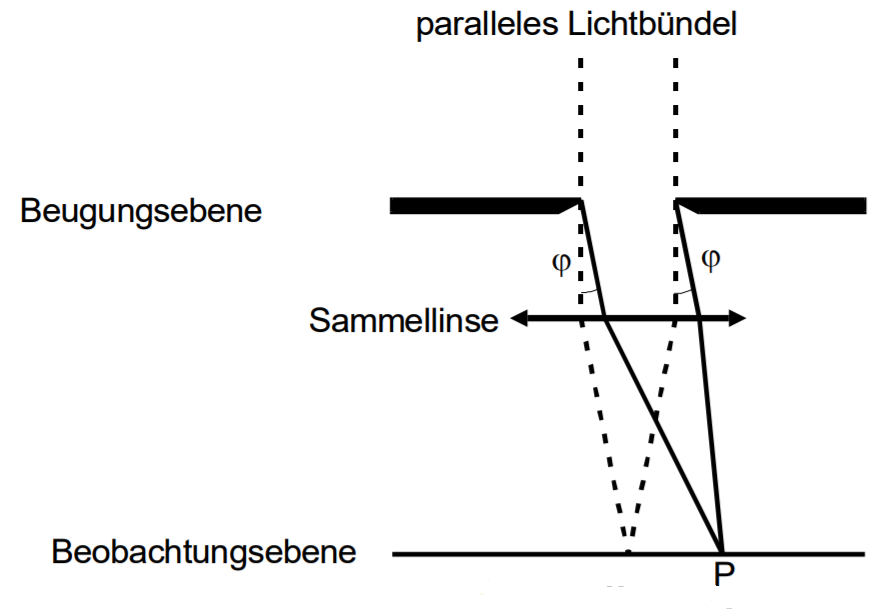
\includegraphics[height=6cm]{data/frau.png}
  \caption{Frauenhofer Beugung an einem Spalt. \cite{sample}}
  \label{fig:frau}
\end{figure}
In diesem Versuch wird nur die Frauenhofer Beugung (siehe Abb. \ref{fig:frau}) betrachtet, da sich diese mathematisch leichter beschreiben lässt als die Fresnel Beugung.
Bei der Frauenhofer Beugung wird angenommen, dass die Lichtquelle und die Beobachtungsebene jeweils unendlich weit von der Beugungsebene entfernt sind.
So kann einerseits das Licht von der Quelle als paralleles Lichtbündel mit einer ebenen Wellenfront aufgefasst werden und
andererseits interferieren in einem Punkt $P$ auf der Beobachtungsebene nur Strahlen die unter dem gleichen Winkel $\phi$ gebeugt werden.
Diese Strahlen besitzen eine Phasendifferenz, die aufgrund des Wegunterschiedes $s$ ensteht (siehe Abb. \ref{fig:phase}).
\begin{figure}
  \centering
  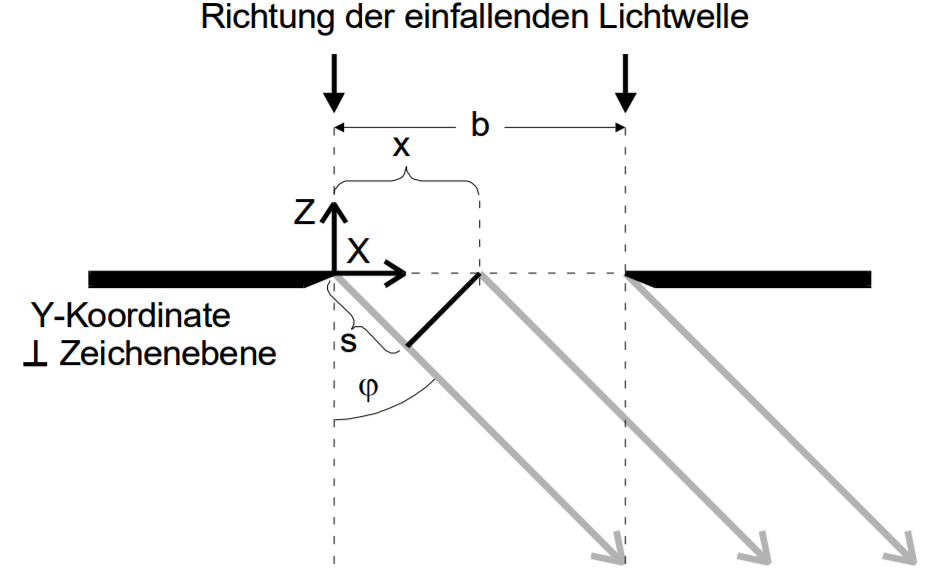
\includegraphics[height=5cm]{data/phase.png}
  \caption{Skizze zur Ableitung der Phasendifferenz. \cite{sample}}
  \label{fig:phase}
\end{figure}
Wenn zwei Strahlen in der Beugungsebene den Abstand $x$ aufweisen, kann mit Abbildung \ref{fig:phase} folgende Phasendifferenz abgeleitet werden:
\begin{equation}
  \delta = \frac{2\pi s}{\lambda} = \frac{2 \pi \sin(\phi)}{\lambda}
  \label{eqn:phase}
\end{equation}
Für die ebene Welle, die sich in $z$-Richtung ausbreitet, wird folgender Ansatz gemacht:
\begin{equation}
  A(z,t) = A_0 e^{\text{i}(\omega t - 2\pi / \lambda)}
\end{equation}
Um nun die Amplitude $B(z,t,\phi)$ eines beliebigen Punktes im Wellenfelds zu erhalten, muss über alle Elementarwellen, die sich in diesem Punkt treffen und überlagern, summiert werden.
Dabei muss die Phasendifferenz aus \eqref{eqn:phase} berücksichtigt werden und da die Elementarwellen eine infinitesimalen Abstand d$x$ haben,
wird die Summe zum Integral über die Spaltbreite $b$.
\begin{equation}
  B(z,t,\phi) = A_0 \int_{0}^{b} \exp\left\{\text{i}\left(\omega t - \frac{2\pi z}{\lambda} + \delta \right)\right\} dx
\end{equation}
\begin{equation}
  B(z,t,\phi) = A_0 \exp\left\{\text{i}\left(\omega t - \frac{2\pi z}{\lambda} \right)\right\} \cdot
  \exp\left\{\text{i}\left( \frac{\pi \text{i} b \sin(\phi) }{\lambda} \right)\right\} \cdot
  \frac{\lambda}{\pi \sin(\phi)} \cdot \sin \left\{ \frac{\pi b \sin(\phi)}{\lambda} \right\}
\end{equation}
Die beiden Exponentialfunktionen beschreiben nur Phasenfunktionen, lediglich die beiden letzten Terme haben einen Einfluss auf Messung des Beugungsbildes.
Statt der Amplitude wird die dazu proportionale Intensität gemessen:
\begin{equation}
  I(\phi) \propto B(\phi)^2 = A_0^2 b^2 \left\{\frac{\lambda}{\pi b \sin(\phi)}\right\}^2 \cdot \sin^2 \left\{ \frac{\pi b \sin(\phi)}{\lambda} \right\}
  \label{eqn:einzel}
\end{equation}
Ein Doppelspalt lässt sich in analoger Form berechnen, wenn er als Überlagerung
zweier Einzelspalte der Breite $b$, die im Abstand $s$ angeordnet sind, betrachtet wird.
Es ergibt sich dann für die Intensitätsverteilung:
\begin{equation}
  I(\phi) \propto B(\phi)^2 = 4 A_0^2 b^2 \cos^2 \left\{ \frac{\pi s \sin(\phi)}{\lambda} \right\} \cdot \left\{\frac{\lambda}{\pi b \sin(\phi)}\right\}^2 \cdot \sin^2 \left\{ \frac{\pi b \sin(\phi)}{\lambda} \right\}
  \label{eqn:doppel}
\end{equation}
Dabei fällt auf, dass die Terme der Intensitätsverteilung des Einzelspaltes wieder auftauchen.
